\chapter{OBJECT DETECTION}

\renewcommand{\headrulewidth}{0.5pt}
\renewcommand{\footrulewidth}{0.5pt}
\thispagestyle{plain}
\pagestyle{fancy}
\fancyhf{}
\fancyhead[L]{\textbf{CHAPTER 2}}
\fancyhead[R]{\textbf{Intelligent Traffic System}}
\raggedright
\fancyfoot[L]{From: ITM Vision}
\fancyfoot[R]{Page \thepage}

\section{Overview}

    \subsection{Traditional Methods}
        Traditional object detection methods are built on handcrafted features and shallow trainable architectures. \\
        \vspace{3mm}
        Features used in traditional methods: color feature, HOG feature, edge feature, optical flow features, texture features,... \\
        \vspace{3mm}
        The pipeline of traditional object detection models can be mainly divided into three stages: informative region selection, feature extraction, and classification.
    
    \subsection{Deep Learning Based Method}

        \subsubsection{CNNs Overview}
            These methods all take advantage of CNN. CNN uses convolutional layers and pooling layers. Convolutional layers filter inputs for useful information. They have parameters that are learned so that filters are adjusted automatically to extract the most useful information for a certain task. Multiple convolutional layers are used that filter images for more and more abstract information after each layer. Pooling layers are used for limited translation and rotation invariance. Pooling also reduces the memory consumption and thus allows for the usage of more convolutional layers. \\
            \vspace{3mm}
            Pooling layers provide an approach to down sampling feature maps by summarizing the presence of features in patches of the feature map. Two common pooling methods are average pooling and max pooling that summarize the average presence of a feature and the most activated presence of a feature respectively. \\
            \vspace{3mm}
            Convolution operation is often interpreted as a filter, where the kernel filters the feature map for information of a certain kind. The convolution operation is usually known as kernels. By different choices of kernels, different operations of the images can be obtained. Operations typically include edge detection, blurring, sharpening etc. A convolutional layer is primarily a layer that performs convolution operation. Its main task is to map. The result of staging convolutional layers in conjunction with the following layers is that the information of the image is classified like in vision. \\
            \vspace{3mm}
            The pooling layer is responsible for reducing the spacial size of the activation maps. Although it reduces the dimensionality of each feature map, it retains the most important information. There are different strategies of the pooling which are max-pooling, average-pooling and probabilistic pooling. \\
            \vspace{3mm}
            After several convolutional and max pooling layers, the high-level reasoning in the neural network is done via Fully Connected Layers (FCLs). A FCL takes all neurons in the previous layer and connects it to every single neuron it has. FCLs are not spatially located anymore, that means they can be visualized as one-dimensional.The sum of output probabilities from the Fully Connected Layer is 1. This is ensured by using the Softmax as the activation function in the output layer of the Fully Connected Layer. \\
            \vspace{3mm}
            A pooling layer is a new layer added after the convolutional layer. Specifically, after a nonlinearity (e.g. ReLU) has been applied to the feature maps output by a convolutional layer; for example the layers in a model may look as follows: \\
                \begin{enumerate}
                    \item Input image
                    \item Convolutional layer
                    \item Nonlinearity
                    \item Pooling layer
                \end{enumerate}

        \subsubsection{Categorize}
            Thanks to Deep Neural Network, a more significant gain is obtained with the introduction of regions with convolutional neural network (CNN) features (R-CNN). DNNs, or the most representative CNNs, act in a quite different way from traditional approaches. They have deeper architectures with the capacity to learn more complex features than the shallow ones. Also, the expressivity and robust training algorithms allow to learn informative object representations without the need to design features manually. \\
            \vspace{3mm}
            Since the proposal of R-CNN, a great deal of improved models have been suggested, including fast R-CNN that jointly optimizes classification and bounding box regression tasks, faster R-CNN that takes an additional subnetwork to generate region proposals, and you only look once (YOLO) that accomplishes object detection via a fixed-grid regression. \\

        \subsubsection{Region Proposal Based Method}
            Generate region proposals at first and then classify each proposal into different object categories. Frameworks may be included such as: R-CNN, Faster R-CNN, region-based fully convolutional network R-FCN, feature pyramid networks (FPN), and Mask R-CNN. \\
            \vspace{3mm}
            Region proposal-based frameworks are composed of several correlated stages, including region proposal generation, feature extraction with CNN, classification, and bounding box regression, which are usually trained separately. Even in the recent end-to-end module Faster R-CNN, an alternative training is still required to obtain shared convolution parameters between RPN and detection network. As a result, the time spent in handling different components becomes the bottleneck in the real-time application. \\

        \subsubsection{Regression / Classification Based Method}
            Regression/classification based framework solves object detection problem by regarding it as regression or classification problem. Some frameworks may be accounted for examples are: MultiBox, AttentionNet, G-CNN, YOLO, Single Shot MultiBox Detector (SSD), YOLOv2, YOLOv3. \\
            \vspace{3mm}
            One-step frameworks based on global regression/classification, mapping straightly from image pixels to bounding box coordinates and class probabilities, can reduce time expense. \\

\section{Comparison YOLO SSD Faster R-CNN}

    \subsection{Faster-RCNN}
        \subsubsection{Architecture}
            The architecture of Faster R-CNN is shown in the next figure. It consists of 2 modules:
            \begin{itemize}
                \item \textbf{RPN:} For generating region proposals. 
                \item \textbf{Faster R-CNN:} For detecting objects in the proposed regions.
            \end{itemize}
            \begin{figure}[H]
                \centering
                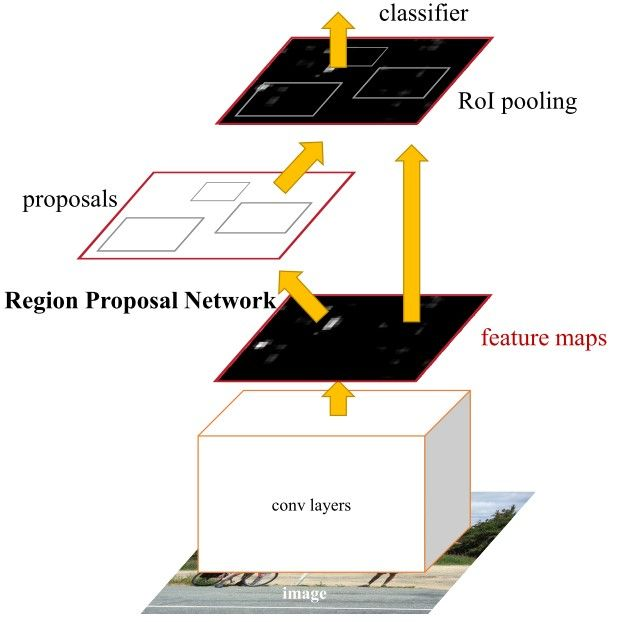
\includegraphics[width=0.6\linewidth]{img/R-CNN.png}
                \caption{Pipeline of Faster R-CNN}
            \end{figure}
        \subsubsection{Region Proposal Generation}
            The RPN module is responsible for generating region proposals. It applies the concept of attention in neural networks, so it guides the Fast R-CNN detection module to where to look for objects in the image. \\ 
            \vspace{3mm}
            The network slides over the conv feature map and fully connects to an n×n spatial window. A low-dimensional vector (512-dimensional for VGG16) is obtained in each sliding window and fed into two sibling FC layers, namely, box-classification layer (cls) and box-regression layer (reg). This architecture is implemented with an n × n conv layer followed by two sibling 1 × 1 conv layers. To increase nonlinearity, ReLU is applied to the output of the n × n conv layer. \\ 
            \vspace{3mm}
            The cls layer outputs a vector of 2 elements for each region proposal. If the first element is 1 and the second element is 0, then the region proposal is classified as background. If the second element is 1 and the first element is 0, then the region represents an object. In other words, it represents a binary classifier that generates the objectness score for each region proposal. \\ 
            \vspace{3mm}
            RPN produces better region proposals compared to generic methods like Selective Search and EdgeBoxes, which are implemented in RCNN and Fast - RCNN. \\ 
            \vspace{3mm}
            The RPN processes the image using the same convolutional layers used in the Fast R-CNN detection network. Thus, the RPN does not take extra time to produce the proposals compared to the algorithms like Selective Search and reduce training time as the RPN and the Fast R-CNN can be merged into a single network.
            \begin{figure}[H]
                \centering
                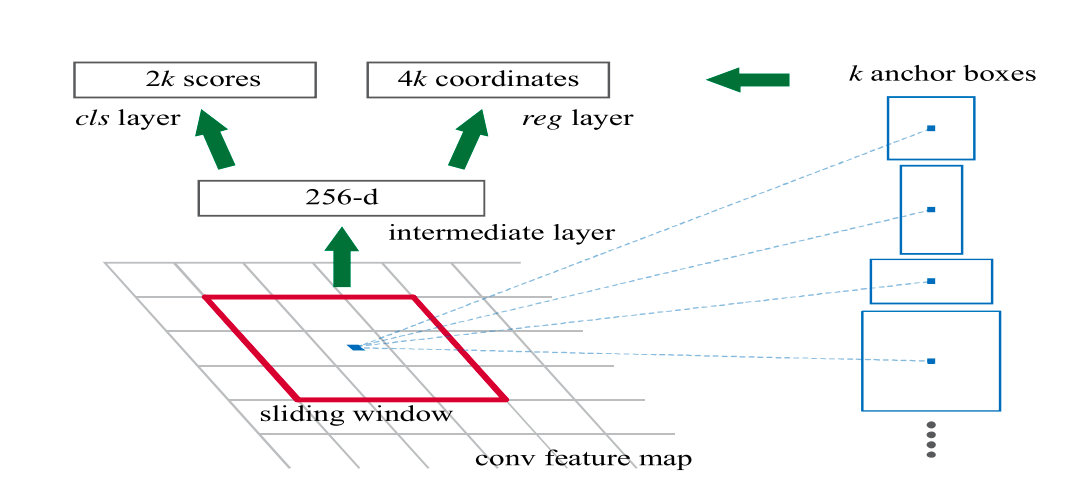
\includegraphics[width=0.6\linewidth]{img/RPN.png}
                \caption{Architecture of RPN}
            \end{figure}
        \subsubsection{Detection Head}
            \begin{enumerate}
                \item \textbf{Anchors} \\ 
                    \vspace{3mm}
                    The feature map of the last shared convolution layer is passed through a rectangular sliding window of size n*n where n = 3 for the VGG-16 net. For each window, K region proposals are generated. Each proposal is parametrized according to a reference box which is called an anchor box. The 2 parameters of the anchor boxes are scale and aspect ratio. Anchors of three scales and three aspect ratios are adopted, therefore K regions are produced from each region proposals. The multi-scale anchors are key to share features across the RPN and the Fast R-CNN detection network. \\ 
                    \vspace{3mm}
                    For training the RPN, each anchor is given a positive or negative \textbf{objectness score} based on the Intersection-over Union (IoU). \\ 
                    \vspace{3mm}
                    The next 4 conditions use the IoU to determine whether a positive or a negative \textbf{objectness score} is assigned to an anchor. Based on this, classification label is produced.
                    \begin{itemize}
                        \item An anchor that has an IoU overlap higher than \textbf{0.7} with any ground-truth box is given a positive objectness label.
                        \item If there is no anchor with an IoU overlap higher than \textbf{0.7}, then assign a positive label to the anchor(s) with the highest IoU overlap with a ground-truth box.
                        \item A negative \textbf{objectness score} is assigned to a \textbf{non-positive} anchor when the IoU overlap for all ground-truth boxes is less than \textbf{0.3}. A negative objectness score means the anchor is classified as background.
                        \item Anchors that are neither positive nor negative do not contribute to the training objective.
                    \end{itemize}
                \item \textbf{Loss Function}
                    \begin{align}
                        L(p_i, t_i) = \frac{1}{N_{cls}} \displaystyle\sum_i L_cls(p_i,p_i\ast) + \lambda \frac{1}{N_{reg}} \displaystyle\sum_i p_i\ast L_{reg} (t_i, t_i\ast)   
                    \end{align}
                    \vspace{3mm}
                    Where $p_i$ is the predicted probability of the $i^{th}$ anchor being an object. The ground truth label $p_i\ast$ is 1 if the anchor is positive, otherwise 0. $t_i$ stores four parameterized coordinates of the predicted boudaring box while $t_i\ast$ is related to the ground truth box overlapping with a positive anchor. $L_cls$ is a binary log loss and $L_reg$ is a smoothed $L_1$ loss. These two terms are normalized with the mini-batch size ($N_cls$) and the number of anchor locations ($N_reg$).
            \end{enumerate}
        \subsubsection{Observations}
            \begin{enumerate}
                \item \textbf{Pros} \\
                    \vspace{3mm}
                    With the proposal of Faster R-CNN, region proposal-based CNN architectures for object detection can really be trained in an end-to-end way.
                \item \textbf{Cons} \\
                    \vspace{3mm}
                    However, the alternate training algorithm is very time-consuming and RPN produces object-like regions (including backgrounds) instead of object instances and is not skilled in dealing with objects with extreme scales or shapes.
            \end{enumerate}

    \subsection{SSD}
        \subsubsection{Feature Extraction}
            SSD uses VGG16 to extract feature maps. VGG16 is a convolutional neural network model proposed by K. Simonyan and A. Zisserman from the University of Oxford in the paper “Very Deep Convolutional Networks for Large-Scale Image Recognition”. The model achieves 92.7\% top-5 test accuracy in ImageNet, which is a dataset of over 14 million images belonging to 1000 classes. It was one of the famous model submitted to ILSVRC-2014. It makes the improvement over AlexNet by replacing large kernel-sized filters (11 and 5 in the first and second convolutional layer, respectively) with multiple 3×3 kernel-sized filters one after another. It is one of the most preferred choices in the community for extracting features from images. The configuration of the VGGNet is publicly available and has been used in many other applications and challenges as a baseline feature extractor.
            \begin{figure}[H]
                \centering
                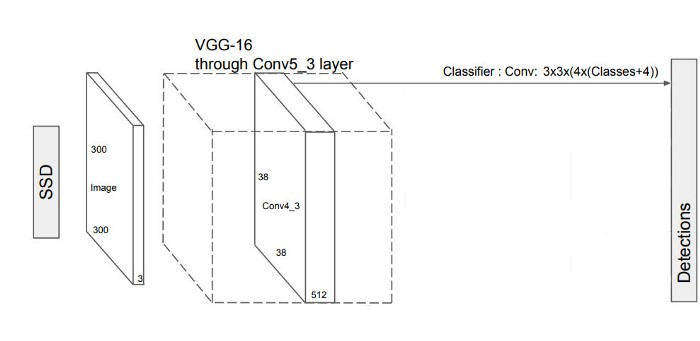
\includegraphics[width=0.6\linewidth]{img/SSD.png}
                \caption{Feature Extractor of SSD}
            \end{figure}
            
            \begin{figure}[H]
                \centering
                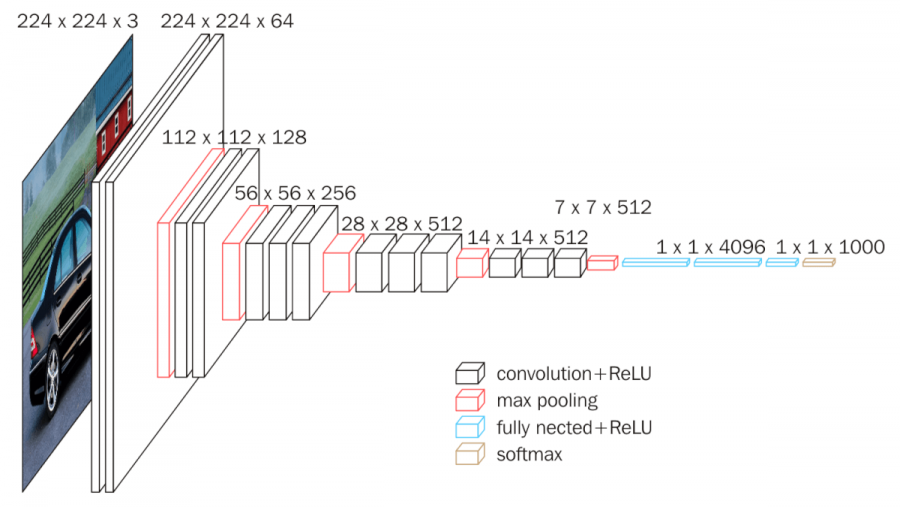
\includegraphics[width=0.6\linewidth]{img/VGG16.png}
                \caption{Architecture of VGG16}
            \end{figure}
        \subsubsection{Multi-scale feature maps for detection}
            Given a specific feature map, instead of fixed grids adopted in YOLO, SSD uses bounding box regression technique,it takes the advantage of a set of default anchor boxes with different aspect ratios and scales to discretize the output space of bounding boxes. To handle objects with various sizes, the network fuses predictions from multiple feature maps with different resolutions. \\ 
            \vspace{3mm}
            SSD adds several feature layers to the end of VGG16 backbone network to predict the offsets to default anchor boxes and their associated confidences. Final detection results are obtained by conducting NMS on multiscale refined bounding boxes.
            \begin{figure}[H]
                \centering
                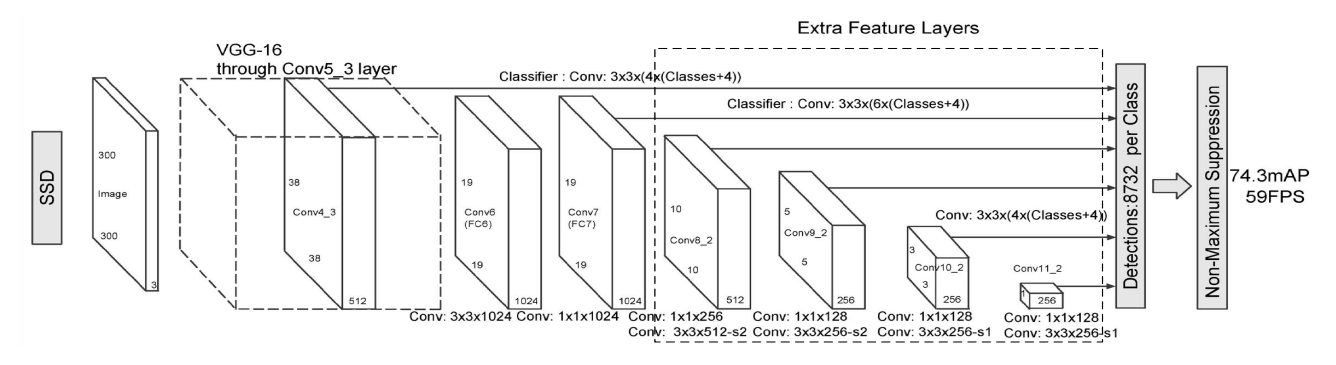
\includegraphics[width=0.6\linewidth]{img/ssd.png}
                \caption{Architecture of SSD}
            \end{figure}
        \subsubsection{Default Boundary Box}
            The default boundary boxes are equivalent to anchors in Faster R-CNN. Default boundary boxes are chosen manually. SSD defines a scale value for each feature map layer. Combining the scale value with the target aspect ratios, we compute the width and the height of the default boxes. For layers making 6 predictions, SSD starts with 5 target aspect ratios: 1, 2, 3, 1/2, and 1/3. Then the width and the height of the default boxes are calculated as:
            \begin{align}
                w = scale.\sqrt{aspect ratio} \\ 
                h = \frac{scale}{\sqrt{aspect ratio}}
            \end{align}
            \vspace{3mm}
            Then SSD adds an extra default box with scale: 
            \begin{align}
                scale = \sqrt{scale.scale at next level}
            \end{align}
            \vspace{3mm}
            Where aspect ratio is equal to 1.
            \begin{figure}[H]
                \centering
                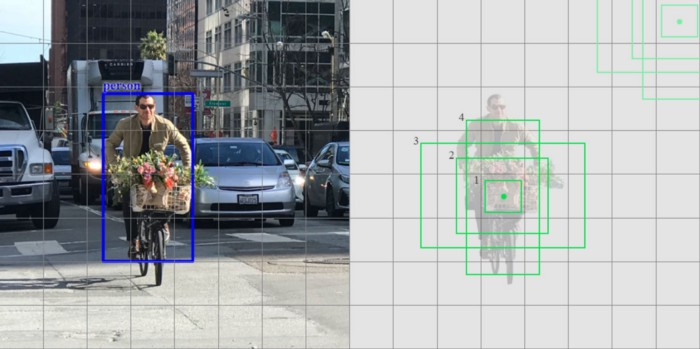
\includegraphics[width=0.6\linewidth]{img/boundary.png}
                \caption{Default Boundary Box}
            \end{figure}
        \subsubsection{Matching Strategy}
            SSD predictions are classified as positive matches or negative matches. SSD only uses positive matches in calculating the localization cost (the mismatch of the boundary box). If the corresponding default boundary box (not the predicted boundary box) has an IoU greater than 0.5 with the ground truth, the match is positive. Otherwise, it is negative. Once we identify the positive matches, we use the corresponding predicted boundary boxes to calculate the cost. This matching strategy nicely partitions what shape of the ground truth that a prediction is responsible for.
            \begin{figure}[H]
                \centering
                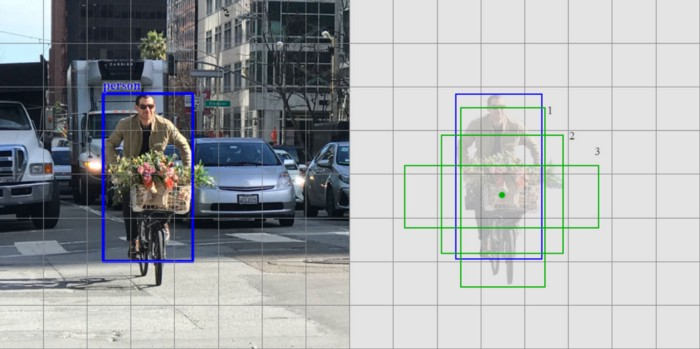
\includegraphics[width=0.6\linewidth]{img/matching.png}
                \caption{Matching with ground truth}
            \end{figure}
        \subsubsection{Loss Function}
            There are two types of loss functions here: Confidence loss and Location loss.
            \begin{itemize}
                \item There are two types of loss functions here: Confidence loss and Location loss. \\
                    \vspace{3mm}
                    The localization loss between the predicted box \textbf{l} and the ground truth box \textbf{g} is defined as the smooth $L_1$ loss with \textbf{$c_x,c_y$} as the offset to the default bounding box \textbf{d} of width \textbf{w} and height \textbf{h}.
                    \begin{align}
                        L_loc(x,l,g) = \displaystyle\sum_{i \in Pos}^{N} \displaystyle\sum_{m \in c_x,c_x,w,h} x_{ij}^k smooth_{L_1} (l_i^m - \hat{g}_j^m) \\ 
                        \hat{g}_j^{c_x} =\frac{(g_j^{c_x} - d_i^{c_x})}{d_i^w} ; \hat{g}_j^{c_y} = \frac{(g_j^{c_y} - d_i^{c_y})}{d_i^h} \\ 
                        \hat{g}_j^w = \log(\frac{g_j^w}{d_i^w}) ; \hat{g}_j^h = \log(\frac{g_j^h}{d_i^h}) \\
                        x_{ij}^p = \left\{ 
                            \begin{array}{ll}
                                1 & \mbox{if IoU > 0.5 between default box i and ground true box j on class p} \\ 
                                0 & \mbox{Otherwise} 
                            \end{array}
                        \right.
                    \end{align} 
                \item The confidence loss is a measure of the confidence that an algorithm quantifies if a bounding box in an image consists of any object or class. For every positive match prediction, we penalize the loss according to the confidence score of the corresponding class. For negative match predictions, we penalize the loss according to the confidence score of the class “0”: class “0” classifies no object is detected.The alpha term balances the contribution of the location losses. The main objective in neural neutral is to analyse the parameters that reduce the loss predictions. \\ 
                    \vspace{3mm}
                    It is calculated as the softmax loss over multiple classes confidences \emph{c} (class score).
                    \begin{align}
                        L_{conf}(x,c) = - \displaystyle\sum_{i \in Pos}^N x_{ij}^p \log(\hat{c}_i^0) where \hat{c}_i^p = \frac{exp(c_i^p)}{(\displaystyle\sum)_p exp(c_i^p)}
                    \end{align}
                    where \emph{N} is the number of matched default boxes.
                \item The final loss function is computed as: 
                    \begin{align}
                        L(x,c,l,g) = \frac{1}{N} (L_{conf}(x,c) + \propto L_{loc}(x,l,g))
                    \end{align}
                    where \emph{N} is the number of positive matches and $\alpha$ is the weight for the localization loss.
            \end{itemize}

        \subsubsection{Hard negative mining}
            SSD still requires negative sampling so it can learn what constitutes a bad prediction. So, instead of using all the negatives, we sort those negatives by their calculated confidence loss. SSD picks the negatives with the top loss and makes sure the ratio between the picked negatives and positives is at most 3:1. This leads to faster and more stable training.

        \subsubsection{Observations}
            \begin{enumerate}
                \item \textbf{Pros} \\ 
                    \vspace{3mm}
                    SSD is a single-shot detector. It has no delegated region proposal network and predicts the boundary boxes and the classes directly from feature maps in one single pass. \\ 
                    \vspace{3mm}
                    To improve accuracy, SSD introduces:
                    \begin{itemize}
                        \item Small convolutional filters to predict object classes and offsets to default boundary boxes.
                        \item Separate filters for default boxes to handle the difference in aspect ratios.
                        \item Multi-scale feature maps for object detection.
                    \end{itemize}
                    \vspace{3mm}
                    SSD can be trained end-to-end for better accuracy. SSD makes more predictions and has better coverage on location, scale, and aspect ratios. With the improvements above, SSD can lower the input image resolution to 300 × 300 with a comparative accuracy performance. Integrating with hard negative mining, data augmentation, and a larger number of carefully chosen default anchors, SSD significantly outperforms the Faster R-CNN in terms of accuracy on PASCAL VOC and COCO while being three times faster.
                \item \textbf{Cons} \\ 
                Shallow layers in a neural network may not generate enough high level features to do prediction for small objects. Therefore, SSD does worse for smaller objects than bigger objects. \\ 
                \vspace{3mm}
                The need of complex data augmentation also suggests it needs a large number of data to train. For example, SSD does better for Pascal VOC if the model is pretrained on COCO dataset.
            \end{enumerate}

    \subsection{YOLO}
        \subsubsection{Network Architecture}
            The whole system can be divided into two major components: Feature Extractor and Detector; both are multi-scale. When a new image comes in, it goes through the feature extractor first so that we can obtain feature embeddings at three (or more) different scales. Then, these features are feed into three (or more) branches of the detector to get bounding boxes and class information.
            \begin{figure}[H]
                \centering
                \includegraphics[width=0.8\linewidth]{img/yolo.png}
                \caption{Major components}
            \end{figure}
        \subsubsection{Feature Extraction}
            The feature extractor YOLO V3 uses is called Darknet-53. Darknet-53 contains 53 layers and borrows the ideas of skip connections to help the activations to propagate through deeper layers without gradient diminishing from ResNet. But the Darknet-53 claims to be more efficient than ResNet101 or ResNet152.
            \begin{figure}[H]
                \centering
                \includegraphics[width=0.8\linewidth]{img/feature_extraction.png}
                \caption{Feature Extraction of YOLOv3}
            \end{figure}
            \vspace{3mm}
            Inside the block, there’s just a bottleneck structure (1x1 followed by 3x3) plus a skip connection. If the goal is to do multi-class classification as ImageNet does, an average pooling and a 1000 ways fully connected layers plus softmax activation will be added. However in the case of object detection, the classification head won't be included, instead, the "detection" head will be added to this feature extractor. Features from last three residual blocks are used in the later detection. 
        \subsubsection{Multi-scale Detector}
            \begin{enumerate}
                \item IOU (Intersection Over Union) \\
                \vspace{3mm}
                Intersection over Union is an evaluation metric used to measure the accuracy of an object detector on a particular dataset. \\
                \vspace{3mm}
                Intersection over Union is a ratio. In the numerator we compute the area of overlap between the predicted bounding box and the ground-truth bounding box The denominator is the area of union, or more simply, the area encompassed by both the predicted bounding box and the ground-truth bounding box. Dividing the area of overlap by the area of union yields our final score — the Intersection over Union. \\
                \vspace{3mm}
                \begin{figure}[H]
                    \centering
                    \includegraphics[width=0.6\linewidth]{img/IOU.png}
                    \caption{IOU formula}
                \end{figure}
                \item Anchor Box \\
                \vspace{3mm}
                The goal of object detection is to get a bounding box and its class. Bounding box usually represents in a normalized xmin, ymin, xmax, ymax format. \\ 
                \vspace{3mm}
                \begin{figure}[H]
                    \centering
                    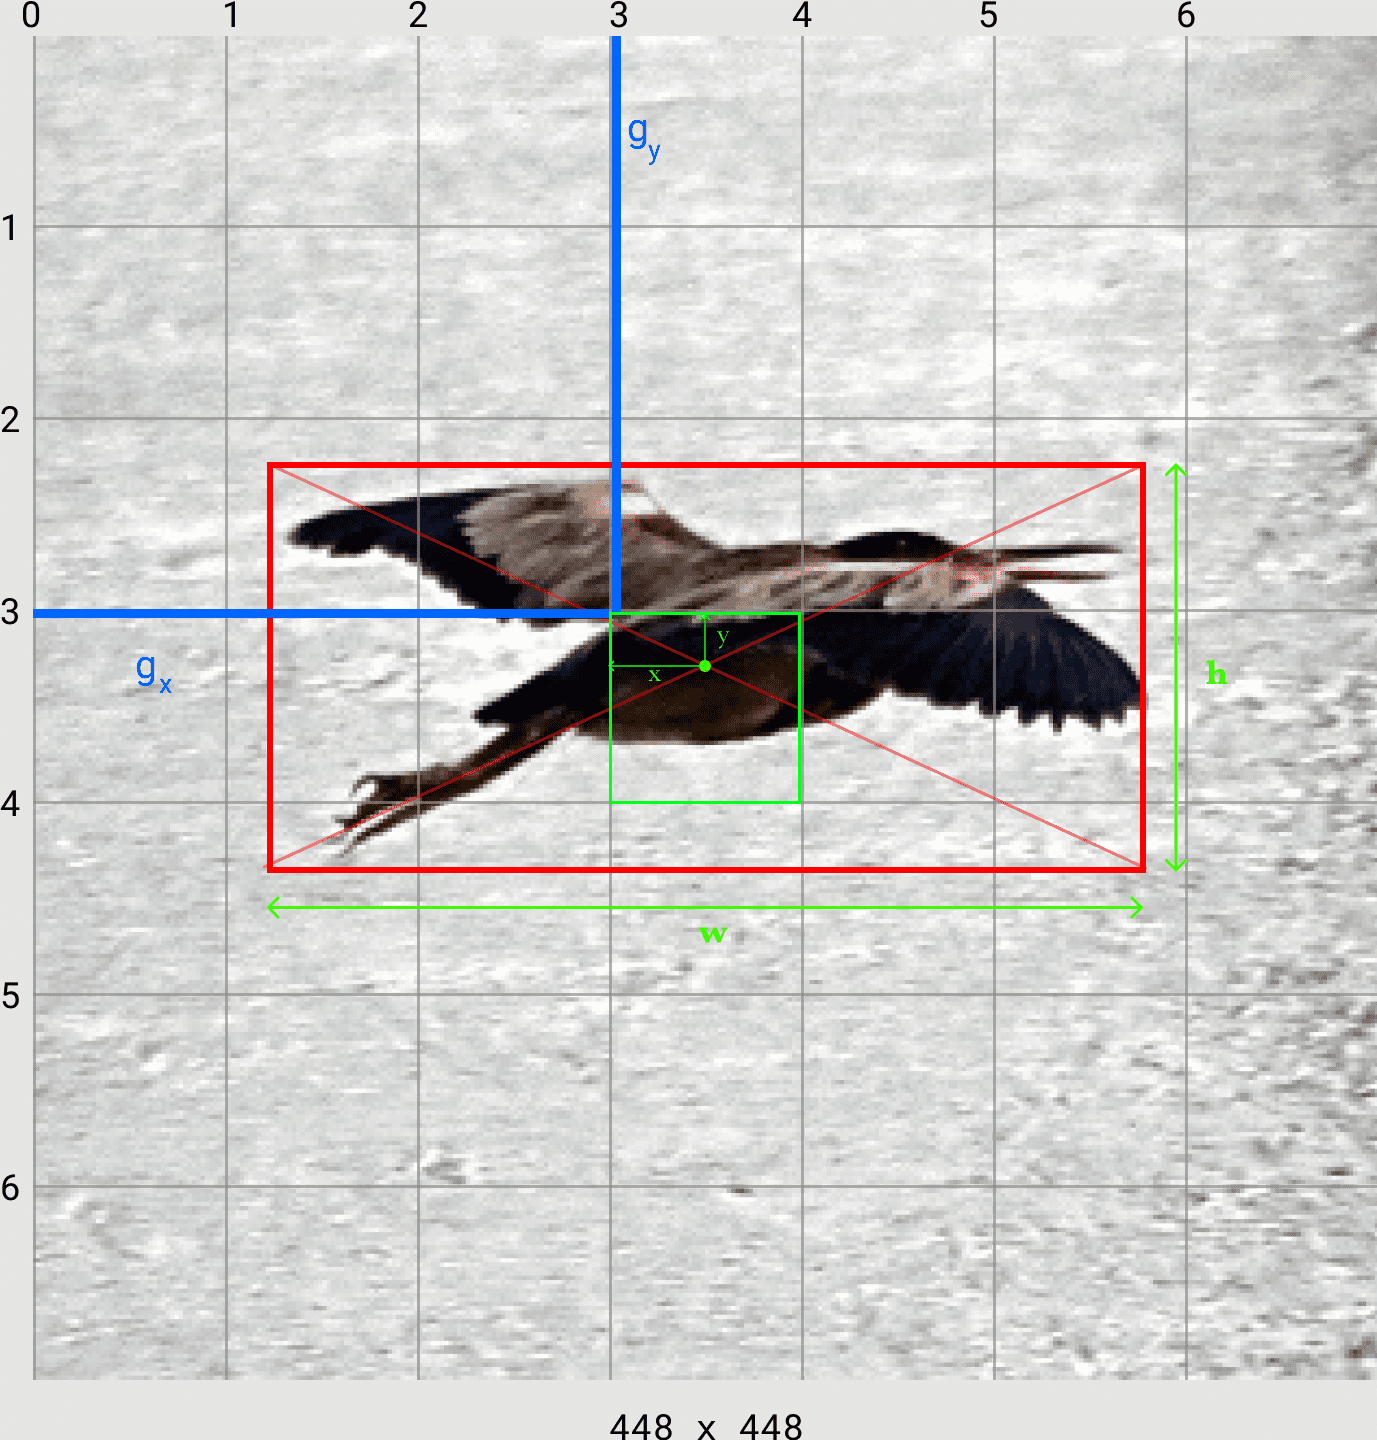
\includegraphics[width=0.6\linewidth]{img/bird.png}
                    \caption{Example for anchor box}
                \end{figure}
                \vspace{3mm}
                The input image is divided into an S x S grid of cells. For each object that is present on the image, one grid cell is said to be “responsible” for predicting it. Anchor boxes are assigned to each cell of the grid.  And once we defined those anchors, we can determine how much does the ground truth box overlap with the anchor box and pick the one with the best IOU and couple them together. \\
                \vspace{3mm}
                In YOLO v3, we have three anchor boxes per grid cell. And we have three scales of grids: \\
                \begin{itemize}
                    \item The location offset against the anchor box: tx,ty,tw,th. This has 4 values.
                    \item The confidence score to indicate if this box contains an object. This has 1 value. The confidence score is defined as $P_{object} * IOU_{pred}^{truth}$ which indicates how likely there is exist objects ($P_{object}\geq0$) and show confidence of its prediction ($IOU_{pred}^{truth}$).
                    \item The conditional class probabilities $P(Class_i|Object)$ to tell us which class this box belongs to. This has number of values according to number of classes.
                \end{itemize}
                \item Loss Function \\
                \vspace{3mm}
                During training the following loss function introduced in YOLO paper is optimize. \\
                \vspace{3mm}
                \begin{align}
                    \lambda_{coord} \displaystyle\sum_{i=0}^{s^2} \displaystyle\sum_{j=0}^{B} \mathbb{1}_{ij}^{obj} [(x_i - \hat{x_i})^2 + (y_i - \hat{y_i})^2] \\
                    \lambda_{coord} \displaystyle\sum_{i=0}^{s^2} \displaystyle\sum_{j=0}^{B} \mathbb{1}_{ij}^{obj} [(\sqrt{w_i} - \sqrt{\hat{w_i}})^2 + (\sqrt{h_i} - \sqrt{\hat{h_i}})^2] \\
                    \displaystyle\sum_{i=0}^{s^2} \displaystyle\sum_{j=0}^{B} \mathbb{1}_{ij}^{obj} (C_i - \hat{C_i})^2 \\ 
                    \lambda_{noobj} \displaystyle\sum_{i=0}^{s^2} \displaystyle\sum_{j=0}^{B} \mathbb{1}_{ij}^{noobj} (C_i - \hat{C_i})^2 \\ 
                    \displaystyle\sum_{i=0}^{s^2} \mathbb{1}_{i}^{obj} \displaystyle\sum_{c \in classes} (p_i(c) - \hat{p_i}(c))^2
                \end{align}
                \vspace{3mm}
                \par The loss function contain 4 parts : centroid loss, anchor box's width and height loss, confidence loss, classification loss. \\
                \vspace{3mm}
                \ding{114}\textbf{Centroid Loss:} the smaller this loss is, the closer the centroids of predictions and ground truth are. Since this is a regression problem, we use mean square error here. Besides, if there're no object from the ground truth for certain cells, we don't need to include the loss of that cell into the final loss. Therefore we also multiple by object mask. Object mask is either 1 or 0, which indicates if there's an object or not. \\ 
                \vspace{2mm}
                \ding{114}\textbf{Anchor's box width and height loss:} this term penalizes the bounding box with inacurate height and width. The square root is present so that erors in small bounding boxes are more penalizing than errors in big bounding boxes. \\ 
                \vspace{2mm}
                \ding{114}\textbf{Confidence loss:} tries to make the confidence score equal to the IOU between the object and the prediction when there is one object or close to 0 when there is no object in the cell. \\ 
                \vspace{2mm}
                \ding{114}\textbf{Classification loss:} is calculated by binary cross-entropy loss. \\
                \vspace{3mm}
                In YOLOv3, they made some modifications to the loss function, confidence loss now uses binary cross-entropy loss to calculated instead of mean square error. The classification loss is now changed into multi-label classification instead of multi-class classification, therefore independent logistic classifiers replaced the softmax for better class prediction.Because some dataset may contains labels that are related to each other.  
            \end{enumerate}
        \subsubsection{Post Processing}
            The final component in this detection system is a post-processor. In YOLO, non maximum suppression is used to eleminate duplicate results.

        \subsubsection{Modifications of YOLO}
            For older version of YOLO, spatial constraint is one major drawback of the algorithm as a grid can analyse only up to two blocks and these two blocks can contain only one class. This results in a reduction in the detection of the nearby objects. It is quite difficult to detect small images in a group image with the help of this algorithm. As it uses the last-stage feature map, which has only the coarse information as it passes through the neural network, the accuracy has a limitation. \\
            \vspace{3mm}
            Bochkovskiy et al proposed the YOLOv4algorithm with significant changes from the previous version, and much better accuracy. Published in April 2020 it is the latest, most advanced iteration of YOLO, and the first developed by the original authors (Redmon et al). To achieve better accuracy, they designed a deeper and complex network, where they used Dense Block. It contains multiple convolutional layers, with batch normalization, ReLU, after which convolution takes place. \\
            \vspace{3mm}
            For the backbone of the feature extraction, they used the CSPDarknet-53, which uses the CSP connections along with Darknet-53 from the previous YOLOv3. Spatial Pyramid Pooling (SPP) is used as the neck over CSPDarknet-53 as it increases the receptive field, differentiates the most significant feature and does not cause a reduction in speed. In place of the Feature Pyramid Network (FPN) in YOLOv3, here they used Path Aggregation Network (PANet). For the head, they used the original YOLOv3 network. \\ 
            \vspace{3mm}
            Apart from the architecture, it consists of a training strategy to get better accuracy without the extra cost to hardware, which is termed as Bag of Freebies. With these, we can get better performance for "free". Another set of strategies which give better results at low cost, but not completely free, were termed as the Bag of Specials. \\ 
            \vspace{3mm}
            With those modification, YOLO is the most commonly used algorithm that is used for detecting natural images as this is the most efficient algorithm for new domains and inputs that are unexpected.
        
    \subsection{Comparision YOLO, SSD and Faster R-CNN}
        \subsubsection{Pascal VOC 2007/2012}
            As YOLO is not skilled in producing object localizations of high IoU, it obtains a very poor result on VOC 2012. However, with the complementary information from Fast R-CNN (YOLO+FRCN) and the aid of other strategies, such as anchor boxes, BN, and fine-grained features, the localization errors are corrected (YOLOv2). 
        \subsubsection{Microsoft COCO}
            Overall, region proposal-based methods, such as Faster R-CNN and R-FCN, perform better than regression/ classification-based approaches, namely, YOLO and SSD, due to the fact that quite a lot of localization errors are produced by regression/classification-based approaches.
        \subsubsection{Time analysis}
            Regression-based models can usually be processed in real time at the cost of a drop in accuracy compared with region proposal-based models. Also, region proposal-based models can be modified into real-time systems.
        \subsubsection{Application in Vehicle Detection System}
            Lecheng Ouyang et al implemented vehicle target detection based on YOLOv3 in complex scenes and showed advantages over traditional target detection algorithms in accuracy and speed. They showed how YOLOv3 can be used for vehicle detection, and it gives an accuracy of 89.16\% at 21fps on the VOC dataset. \\ 
            \vspace{3mm}
            Jeong-ah Kim et al has put three algorithm into test by the the vehicle type classification for the vehicle type recognition was based on the classification of the Korea Expressway Corporation. They found out that Faster R-CNN may not suitable for real-time application, SSD's accuracy is low and sometimes fails to detect a vehicle while YOLOv4 yeilds the most efficient results.[7] \\ 
        \subsubsection{Other Experiments}
            Deepa et al compared all three models for real-time tennis ball tracking and from their work, they concluded that SSD is much efficient and comparatively more accurate accurate algorithm with less computation speed for this particular task of detecting the tennis ball tosses. It worth noticing that, the YOLO version they used is version 1, which performs badly with small objects like tennis ball. This is no longer a shortage to the latest version of YOLO [6]. \\ 
            \vspace{3mm}
            According to [**], when they compared the YOLOv3 algorithm with the SSD, it was shown by evaluation that YOLOv3 had better performance than SSD. If the SSD has an input resolution at 300*300, it would have the same inference as the YOLOv3 at the input resolution 416*416, the precision of YOLOv3 is higher. YOLOv3 is faster than SSD, which is applicable to real-time. \\ 

\section{Metrics and Evaluations}

